

\documentclass[10pt, conference, compsocconf]{IEEEtran}

\ifCLASSINFOpdf

\else

\fi

\usepackage{hyperref}
\usepackage{amsmath}
\usepackage{amssymb}
\usepackage{hhline} % easy to manage table borders
\usepackage{colortbl} % colored cells in tables
\usepackage{multirow}
\usepackage{enumerate}
\usepackage{slashbox} % cell with slash inside
\usepackage{makeidx}  % allows index generation
\usepackage[utf8]{inputenc}
\usepackage{graphicx}

\newtheorem{definition}{Definition}
\newtheorem{example}{Example}

\def\sectionautorefname{Section}
\def\subsectionautorefname{Section}


% correct bad hyphenation here
\hyphenation{op-tical net-works semi-conduc-tor}


\begin{document}

% paper title
% can use linebreaks \\ within to get better formatting as desired
\title{Pharmer -- Semantic Authoring of Medical Prescriptions}
%\title{Pharmer: A platform for health care providers to use linked open data in e-prescriptions}


% author names and affiliations
% use a multiple column layout for up to two different
% affiliations

\author{\IEEEauthorblockN{Ali Khalili}
\IEEEauthorblockA{Faculty of Computer Science\\
University of Leipzig\\
Leipzig, Germany\\
khalili@informatik.uni-leipzig.de}
\and
\IEEEauthorblockN{Bita Sedaghati}
\IEEEauthorblockA{Institute of Pharmacy\\
University of Leipzig\\
Leipzig, Germany\\
bita.sedaghati@uni-leipzig.de}
}


% make the title area
\maketitle

\begin{abstract}
The abstract goes here. DO NOT USE SPECIAL CHARACTERS, SYMBOLS, OR MATH IN YOUR TITLE OR ABSTRACT.

\end{abstract}

\begin{IEEEkeywords}
component; formatting; style; styling;

\end{IEEEkeywords}


\IEEEpeerreviewmaketitle



\section{Introduction}
This is a test \cite{Khalili2012}.

\section{Semantic Content Authoring}
\label{sec:sca}

\section{E-Prescriptions}
E-health has evolved and emerged recently in many forms. 
E-prescription is one of these forms and is a computer-generated prescription utilized by healthcare providers.
It plays an important role in improving the quality of patient care.
While even nowadays traditional paper prescriptions are commonly used, electronic prescriptions offer several advantages.
As reported in \cite{} medication errors are the most common type of medical error in health care.
In an E-prescription system, prescriber electronically sends an accurate, error-free and understandable prescription directly to a pharmacy from the point-of-care.
Improved confidentiality and security of health information, better clarity and communication among health care providers as well as rapid information exchange are part of arguments for spreading this system.
Reduction in medication error and decline in adverse drug events are more highlighted consequences of E-prescribing.

It is also evident by using the E-prescription, follow up of patient individuals is convenient.
The health care providers can access to the patient's profile and the transfer of these data can appropriately be done.
Besides, the data of medicines consumption and the connection between diagnosed disease and the treatment regimen is recorded.
Furthermore, patient's fate after the medication duration can be followd up by physicians and pharmacists.
The E-prescription information is  of crucial importance as an  informative source for researchers.
Many researchers investigate the aformentioned statistical data and combine them with the information recieved from the medicine producers (e.g. to compare the special drug consumptionin different  individual age ranges).

During the recent years, the adoption of E-prescriptios has been spreading rapidly. 
To illustrate, the Australian government started launching of e-prescription from 1 March 2007.
Using this system, the e-providers who effectively market themselves on the web will have a distinct advantage\cite{Ravichandran}.
A system called epSOS perform the use of E-prescritions all around europe, is currently passing the extensive practical testing phase.
It contains patient summery and E-Prescription Service which allows access to the cross-border eHealth services when seeking healthcare in participating epSOS pilot countries, as tourists, business travellers, commuters or exchange students.
The E-Prescribing Incentive Program is performed in US as a reporting program that uses a combination of incentive payments and payment adjustments to encourage electronic prescribing by eligible professionals.

There are challenges that are solved by E-prescription systems.
Once writing a prescription it is very critical to consider drug interactions. 
Drug interactions are devided to three categories namely \emph{food-drug}, \emph{drug-drug} and \emph{drug-plant} interactions.
Coadministration can either be synergistic or antagonistic which respectively increase or decrease the drugs effect. 
The interactions may sometimes lead to change in the drug effect.
By applying E-prescription system, all types of drug interactions are prevented and the probability of errors in prescriptions are reduced to a great extend.
A E-prescription simply contains drug information and precautions which are necessary to be considered from patient's side.

One of the most important advantages of E-prescribing is that the connection of physician, pharmacist, patient and pharmacetical researchers and statision.
Once the E-prescription is written by a physician, pharmacist has also access to the prescription.
while the physicion is aware, pharmacist can comment on the prescription content.
The online system is also available for patients who can inquire about any necessary information. 
helath care providers can follow up the patient's treatmet fate. 
The data base of the patients profile in subject of many statistics researchs. 
Besides, researchers are able to conveniently follow the drug in the clinical trial phase.


Another challenge points 

 and needs to be more carfully investigated by health care providers. 



\section{Semantic Authoring of Medical Prescriptions}

\section{Pharmer}
In \autoref{fig:lod}, you can see..
We discussed sth in \autoref{sec:sca}.

\subsection{Architecture}

\begin{figure}[tb]
	\centering
		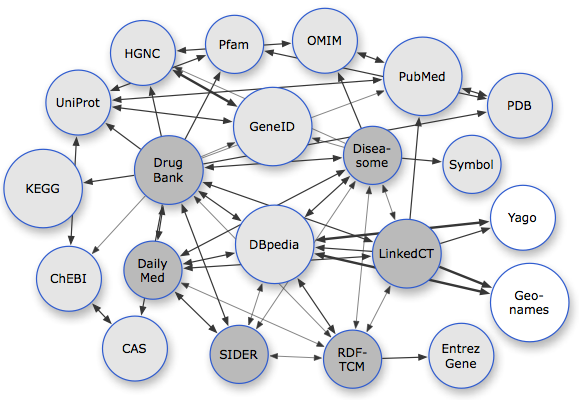
\includegraphics[width=1.0\columnwidth]{images/lod_cloud.png}
	\caption{Available datasets related to pharmaceutical research.}
	\label{fig:lod}
\end{figure}


\section{Conclusion}
The conclusion goes here. this is more of the conclusion

% conference papers do not normally have an appendix


% use section* for acknowledgement
\section*{Acknowledgment}


The authors would like to thank...
more thanks here

\bibliographystyle{IEEEtran}
% argument is your BibTeX string definitions and bibliography database(s)
\bibliography{refs}





% that's all folks
\end{document}


